\subsection{Overview}
Increasingly, internet users are utilizing multiple devices to assist with their daily tasks. According to a study by Criteo\cite{Criteo}, 31\% of purchases involve the use of multiple devices. Users tend to review a product several times from different devices before making a purchase decision. Consequently, company owners, website and app developers have become interested in cross-device tracking to enhance conversion rates and gain deeper insights into consumer behavior. In our research, we aim to explain what cross-device tracking is, its purpose, the potential risks it poses to website users, and demonstrate its usage through practical examples. Additionally, we will compare two categories of websites to identify signs of cross-device tracking implementation.

\subsubsection{Definition}
Cross-device tracking is the process of monitoring user behavior across various devices, such as PCs, smartphones, and tablets, to create the most comprehensive user profile possible by gathering as much information about the user as possible. There are different types of cross-device tracking, which will be described in more detail in Chapter 1.3.

It should be noted that in the modern world, the scope of cross-device tracking is expanding, for instance, with the use of smart homes, as the number of devices increases over time, allowing this technology to be integrated into all areas of a user's life. Additionally, with the development of artificial intelligence, this technology is becoming increasingly precise in recognizing information about users.

\subsubsection{Purpose}
One of the primary reasons companies are exploring cross-device tracking is to improve their marketing strategies and make their advertising more targeted, which is used by a lot of businesses and companies that make marketing analytics.\cite{wizalyArticle} By understanding their customers better through a more complete profile, which includes their activities across multiple devices, companies can more accurately predict both immediate and future buying habits. This not only allows for better-customized advertising that resonates with specific user groups but also helps companies save money by not wasting resources on ineffective ads. While this technology is not universally used yet, its adoption is growing among many companies\cite{CrossDeviceComments}.

Adobe's Cross-Device Analytics, a feature of Adobe Analytics, is a great example of using and implementing this technology. It offers a user-centric view, linking a user's activities across multiple devices like smartphones, tablets, and computers. Key features include Field-Based Stitching, which connects user activities on different devices based on deterministic methods, and Device Graph, which analyzes connections between devices. This helps in attributing user actions accurately, such as linking an ad click on one device to a purchase on another, offering valuable insights for marketing strategies while considering user privacy\cite{CrossDeviceAnalytics}.

However, sales are not the only area where cross-device tracking can be useful. It's also an excellent resource for political parties or media outlets to find their audience, tailoring the right messages or news to specific target groups. The principle is the same: the more information you have about a user, the easier it is to tailor your approach to them. The more sources of information (i.e., devices), the more you can track the behavior and interests of the user.
\subsection{Importance in Modern Digital Exosystem}

\subsubsection{Evolution of User Behavior}
The digital landscape has seen a major evolution in user behavior, particularly in the way people interact with technology. In the early stages of the internet, user behavior was device-specific, primarily bounded to desktop computers. This era was characterized by more predictable online activities, with users typically accessing the internet from fixed locations and a small amount of different devices, which made user tracking relatively easy.

\vspace{0.8cm}
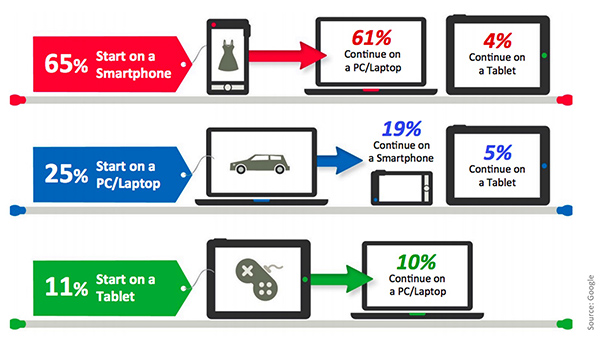
\includegraphics[width=0.95\textwidth]{./assets/google-cdt-stats.jpeg}
\vspace{0.8cm}

The invention of mobile technologies, especially smartphones changed online activities significantly and lead to a transformation in user behavior. Users began interacting with digital content across multiple platforms and often seamlessly switching between devices. For reference, Google published an interesting statistic, that shows more than 80 percent of all users switching their device during the user journey. Multi-platform interaction introduced a new level of complexity in understanding user behavior as users were no longer restricted to a single device.

Moreover, the rise of smart devices and the Internet of Things in the last years are the reason for  even more complex interactions between devices. Today, a wide network of connected devices are creating a diverse and complex digital footprint.

\subsubsection{Challenges in User Tracking}
Parallel to the evolution of users online behavior, the task of tracking users across multiple devices has become increasingly challenging. As there exists no universal login system or consistent identifiers across different websites, establishing a meaningful user profile from disparate device usage is really complex.

Privacy considerations make cross-device tracking even more complicated. With increasing sensitivity to data privacy and the introduction of strong regulations like the General Data Protection Regulation (GDPR) and the California Consumer Privacy Act (CCPA), tracking users across devices must navigate the line between effective data collection and respect for user privacy and consent.

The diversity of devices and platforms results in fragmented data sources, requiring advanced technological solutions for data integration and analysis. The need for algorithms and technologies is necessary to not only gather but also accurately interpret the large amount of data generated by multi-device usage.

Looking ahead, these challenges will even intensify with the continuous evolution of technology. The integration of artificial intelligence and machine learning will potentially lead to advancements in user tracking, but also brings additional complexities regarding privacy regulations. The task of user tracking demands innovative solutions that are adaptable, take privacy into account and are able of decoding increasingly complex device interactions.

\subsubsection{Previous Research}
There are several previous studies\cite{CdtMeasurements,CdtPrivacyAnalysis} that have looked at online data collection, including third-party data collection in the context of cross-device tracking, but as far as we know, the most recent ones are from 2017. In addition, there are also papers \cite{PersonalDataSharing} that focus only on third-party data collection via mobile applications, but we did not find any work that includes mobile and desktop devices. Finally, some researchers have looked at tracking mechanisms that are not cookie-based, such as Flash cookies\cite{FlashCookies}, which are data files created by Adobe Flash that are stored on a users computer making it hard for us to track. Our work focuses primarily on how often websites connect to third-party services and which third-party services they connect to as well as examining indicators relating to cross device tracking

\subsection{Techniques Employed in CDT}
To begin working on the practical part of the project and to better understand which features and traces of cross-device tracking to look for in our collected data, it's necessary to have an understanding of the types of tracking that exist, how companies use them, and what distinguishes them. This will be explored in this chapter.

\subsubsection{Deterministic Tracking}
The most reliable and accurate form of cross-device tracking is deterministic tracking, as it employs verified and identifiable information to associate a user's activities across various devices. This includes unique user data enabling authentication on websites, such as login credentials like email addresses. When a user logs into a website or application with the same credentials on a smartphone, tablet, and laptop, deterministic tracking uses this specific action to link these activities to a unified user profile. Companies can also share identifying information with third parties that do not have direct relationships with the consumer, allowing these entities to participate in cross-device tracking. For instance, websites might transmit identifying information at login to a tracking company, enabling it to match user profiles across different devices. The transmitted information could be the login credentials themselves (for example, an email address) or a cryptographic hash of the identifier.\cite{CdtMeasurements}
The advantage of this cross-device tracking type is its high precision. This method is particularly crucial for our study because, unlike other types, its characteristics and traces can be detected.In the course of our project, the examination of certain websites showed the inherent risks associated with deterministic tracking. These observations have prompted a deeper reflection on the balance between the benefits of precise user tracking and the user privacy. The ethical implications and potential privacy risks highlighted by these findings will be explored and discussed in Chapter \ref{sec:results}. This discussion aims to contribute to the ongoing dialogue on digital privacy and the ethical use of user data in cross-device tracking.

\subsubsection{Probabilistic Tracking}
Probabilistic cross-device tracking emerges as the second primary method for analyzing consumer behavior across various devices, utilizing statistical algorithms to predict the association of different devices with a single user. This method analyzes huge volumes of anonymized data, such as device types, operating systems, and online behavior patterns, to establish connections between devices and users\cite{LiuZhang2021}. Following extensive analysis, probability graphs and other data visualizations are compiled for marketing analysis.

One of the main advantages of probabilistic tracking is its scalability and flexibility. Unlike deterministic tracking, which requires precise identifiers, the probabilistic method can cover a much wider range of devices and users. This makes it particularly effective in situations where direct login data is unavailable. Moreover, the anonymous nature of the collected data can reduce privacy concerns, which is especially important in fields where a lot of sensitive data is present.

However, the probabilistic method has its disadvantages. The main issue lies in accuracy: without the use of specific identifiers, there is always a possibility of error in matching devices to users. This uncertainty can lead to inaccuracies in advertising personalization and consumer behavior analysis. Furthermore, despite the anonymity of the collected data, the extensive collection and analysis of information can raise concerns among users who may not be aware of such tracking. Finally, the complexity of the algorithms and the need to process large volumes of data make probabilistic tracking a technically challenging task, requiring a lot of time and resources for implementation.\cite{FTC} 

\subsubsection{Other methodologies}
In addition to deterministic and probabilistic tracking, there are other techniques and approaches that significantly expand the capabilities of marketers and analysts.

One of the techniques is browser fingerprinting, which involves collecting a set of information associated with a user's device, ranging from hardware specifications to the operating system, browser type and its configuration. It's a process of collecting data through a web browser to create a unique fingerprint of the device. By running a simple script within the browser, a server can gather a wide range of information from public interfaces known as Application Programming Interfaces (APIs) and HTTP headers. APIs serve as interfaces providing access to specific objects and functions. Unlike cookies, which rely on a unique identifier stored directly in the browser, browser fingerprinting is considered entirely stateless. It leaves no traces as it doesn't require saving information within the browser.\cite{Laperdrix2019BrowserFingerprinting}

Also cookies play a really important role in modern cross device tracking by allowing websites to store information about visitors and their preferences. This enables the personalization of the user experience and the delivery of advertising based on the user's previous interactions with the web-site. In cross-device tracking, cookies can be utilized to gather data on user behavior across different devices, enabling advertisers and webmasters to create a unified user profile. This facilitates more targeted and effective advertising, as well as improving analytics and understanding user patterns. Despite their popularity and usefulness, the use of cookies raises concerns about data privacy and security. Users are becoming  aware of how their data is collected and used, demanding more control over their personal information. This has led to the tightening of legislation, such as the General Data Protection Regulation (GDPR) in the European Union and the California Consumer Privacy Act (CCPA), aimed at protecting user rights and privacy protection.\cite{Mitchell2013ThirdPartyCookies}

Of course all of these methods are used simultaneously, allowing for improved data collection and compensating for the limitations of each method. With the improvement of technology, new cross-device tracking methods are implemented, including the use of artificial intelligence and machine learning for deeper analysis of behavioral patterns, as well as the development of new approaches to device and user identification.

